\cleardoublepage

\chapter{Sides}

%%%%%%%%%%%%%%%%%%%%%%%%%%%%%%%%%%%%%%%%%%%%%%%%%%%%%%%%%%%%%%%%%%%%%%%%%%%
%%%%%%%%%%%%%%%%%%%%%%%%%%%%%%%%%%%%%%%%%%%%%%%%%%%%%%%%%%%%%%%%%%%%%%%%%%%
%%%%%%%%%%%%%%%%%%%%%%%%%%%%%%%%%%%%%%%%%%%%%%%%%%%%%%%%%%%%%%%%%%%%%%%%%%%
%%%%%%%%%%%%%%%%%%%%%%%%%%%%%%%%%%%%%%%%%%%%%%%%%%%%%%%%%%%%%%%%%%%%%%%%%%%
%%%%%%%%%%%%%%%%%%%%%%%%%%%%%%%%%%%%%%%%%%%%%%%%%%%%%%%%%%%%%%%%%%%%%%%%%%%

\section{Présentation}

\textit{Sides} est un projet de gestion de titres développé par Sopra Group, plus particulièrement par l'agence de Clermont Ferrand.
Il permet de produire des passeports ou des cartes d'identités pour une dizaine de différents gouvernement comme les Philippines, la Lituanie, la Belgique, Monaco, \ldots
\\

Pour chacun des pays et titres, une application a été développée.
Plutôt que de redévelopper la même application, un nouveau projet a vu le jour : \textit{SITI}.
Cette solution pourra ensuite être vendue à divers pays sans avoir à la ré-implémenter à nouveau.

Actuellement l'équipe Sides n'effectue que de la tiers maintenance applicative (TMA) sur les différentes applications existantes.
L'objectif est de corriger les bugs éventuels ou d'ajouter de nouvelles fonctionnalités.

%%%%%%%%%%%%%%%%%%%%%%%%%%%%%%%%%%%%%%%%%%%%%%%%%%%%%%%%%%%%%%%%%%%%%%%%%%%
%%%%%%%%%%%%%%%%%%%%%%%%%%%%%%%%%%%%%%%%%%%%%%%%%%%%%%%%%%%%%%%%%%%%%%%%%%%
%%%%%%%%%%%%%%%%%%%%%%%%%%%%%%%%%%%%%%%%%%%%%%%%%%%%%%%%%%%%%%%%%%%%%%%%%%%
%%%%%%%%%%%%%%%%%%%%%%%%%%%%%%%%%%%%%%%%%%%%%%%%%%%%%%%%%%%%%%%%%%%%%%%%%%%
%%%%%%%%%%%%%%%%%%%%%%%%%%%%%%%%%%%%%%%%%%%%%%%%%%%%%%%%%%%%%%%%%%%%%%%%%%%

\section{Chargement d'empreintes}

%%%%%%%%%%%%%%%%%%%%%%%%%%%%%%%%%%%%%%%%%%%%%%%%%%%%%%%%%%%%%%%%%%%%%%%%%%%
%%%%%%%%%%%%%%%%%%%%%%%%%%%%%%%%%%%%%%%%%%%%%%%%%%%%%%%%%%%%%%%%%%%%%%%%%%%
%%%%%%%%%%%%%%%%%%%%%%%%%%%%%%%%%%%%%%%%%%%%%%%%%%%%%%%%%%%%%%%%%%%%%%%%%%%

\subsection{Contexte}

L'application Sides à destination de la Lituanie permet la gestion de passeports.
Ces passeports nécessitent la lecture des empreintes du porteur pour être valides.
Lorsque les porteurs sont des personnes diplomatiques ou haut placées, celles-ci désireraient ne pas perdre de temps lors de création ou renouvellement de titres.

Pour satisfaire ces exigences, une personne du gouvernement munie d'un ordinateur portable, de l'application Sides et du périphérique va effectuer la saisie des empreintes sur le lieu désiré : ville plus proche, lieu de travail, \ldots

%%%%%%%%%%%%%%%%%%%%%%%%%%%%%%%%%%%%%%%%%%%%%%%%%%%%%%%%%%%%%%%%%%%%%%%%%%%
%%%%%%%%%%%%%%%%%%%%%%%%%%%%%%%%%%%%%%%%%%%%%%%%%%%%%%%%%%%%%%%%%%%%%%%%%%%
%%%%%%%%%%%%%%%%%%%%%%%%%%%%%%%%%%%%%%%%%%%%%%%%%%%%%%%%%%%%%%%%%%%%%%%%%%%

\subsection{Contrôle de la date}

La première version de cette fonctionnalité permettait l'importation des empreintes les plus récentes présentes dans la base de données pour créer un nouveau passeport.
Les empreintes peuvent venir d'une ancienne demande ou avoir été saisies pour une personne diplomatique comme expliqué précédemment.

Pour sécuriser l'application et le chargement d'anciennes empreintes, l'évolution de la fonctionnalité a pour objectif de contrôler la date d'importation des empreintes dans la base de données.
\\

Pour réaliser ce contrôle, j'ai dû étudier le fonctionnement de l'application pour comprendre le processus de chargement des empreintes dans une nouvelle demande de passeport.

%%%%%%%%%%%%%%%%%%%%%%%%%%%%%%%%%%%%%%%%%%%%%%%%%%%%%%%%%%%%%%%%%%%%%%%%%%%
%%%%%%%%%%%%%%%%%%%%%%%%%%%%%%%%%%%%%%%%%%%%%%%%%%%%%%%%%%%%%%%%%%%%%%%%%%%
%%%%%%%%%%%%%%%%%%%%%%%%%%%%%%%%%%%%%%%%%%%%%%%%%%%%%%%%%%%%%%%%%%%%%%%%%%%
%%%%%%%%%%%%%%%%%%%%%%%%%%%%%%%%%%%%%%%%%%%%%%%%%%%%%%%%%%%%%%%%%%%%%%%%%%%
%%%%%%%%%%%%%%%%%%%%%%%%%%%%%%%%%%%%%%%%%%%%%%%%%%%%%%%%%%%%%%%%%%%%%%%%%%%

\section{Les certificats}

%%%%%%%%%%%%%%%%%%%%%%%%%%%%%%%%%%%%%%%%%%%%%%%%%%%%%%%%%%%%%%%%%%%%%%%%%%%
%%%%%%%%%%%%%%%%%%%%%%%%%%%%%%%%%%%%%%%%%%%%%%%%%%%%%%%%%%%%%%%%%%%%%%%%%%%
%%%%%%%%%%%%%%%%%%%%%%%%%%%%%%%%%%%%%%%%%%%%%%%%%%%%%%%%%%%%%%%%%%%%%%%%%%%

\subsection{Contexte}

La gestion des identités de personnes, au niveau national, est un domaine très sensible qui requière une sécurité élevée des systèmes informatiques.
La solution permettant de sécuriser les données consiste à chiffrer ou signer les données échangées, garantissant ainsi que les données ne pourront être découverte ou qu'elles n'ont pas été modifiée ou envoyées par une personne tiers. Ce chiffrement s'effectue grâce à des certificats.

%%%%%%%%%%%%%%%%%%%%%%%%%%%%%%%%%%%%%%%%%%%%%%%%%%%%%%%%%%%%%%%%%%%%%%%%%%%
%%%%%%%%%%%%%%%%%%%%%%%%%%%%%%%%%%%%%%%%%%%%%%%%%%%%%%%%%%%%%%%%%%%%%%%%%%%
%%%%%%%%%%%%%%%%%%%%%%%%%%%%%%%%%%%%%%%%%%%%%%%%%%%%%%%%%%%%%%%%%%%%%%%%%%%

\subsubsection{Le chiffrement}

Pour assurer que personne ne puisse découvrir le message échangé entre deux personnes il est nécessaire de les chiffrer.

Cette méthode utilise deux entités : un couple de clés composé d'une clé publique ($K$) et d'une clé privée ($K'$), et un algorithme mathématique composé d'une fonction ($F$) et de sa réciproque ($F'$).
Le chiffrement consiste à utiliser une clé dans l'algorithme, et le déchiffrement à utiliser la fonction inverse avec l'autre clé pour retrouver les données d'origine, comme le résume la fonction suivant :
\[
F_K[\ F_{K'}(M)\ ] = M = F'_{K'}[\ F_K(M)\ ]
\]
\\

Le fonctionnement de l'échange d'un message chiffré est le suivant, schématisé par la figure \ref{chiffrement} :
\begin{enumerate}
	\item Bob possède une paire de clé publique/privée, et Alice désire envoyer un message à Bob ;
	\item Bob envoie sa clé publique à Alice ;
	\item Alice chiffre son message grâce à cette clé publique ;
	\item Alice envoie ensuite son message chiffré à Bob ;
	\item Bob déchiffre le message chiffré grâce à sa clé privée. Personne d'autre ne peut le faire car il est le seul à posséder la clé privée.
\end{enumerate}
\begin{figure}[!h]
	\center
	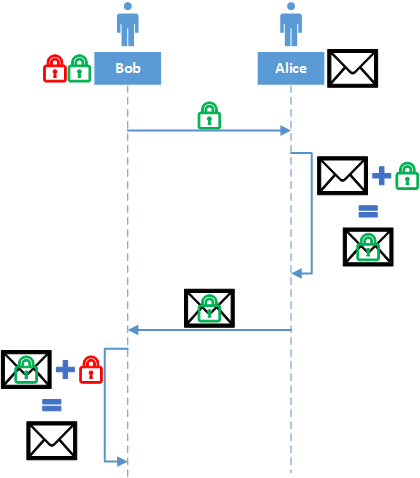
\includegraphics[width=0.7\textwidth]{img/chiffrement.png}
	\caption{Échange d'une message chiffré}
	\label{chiffrement}
\end{figure}
~~\\

La sécurité est basée sur deux principes : le chiffrement et la confidentialité.

Si l'algorithme de chiffrement est trop faible alors il sera possible de déchiffrer les données par calcul mathématiques.
De plus, si la clé de chiffrement est trop petite alors la méthode "brute force", consistant à essayer toutes les combinaisons possibles, permettra aussi le déchiffrement

Si la clé privée du certificat est découverte alors les données seront instantanément déchiffrées, ainsi que les futurs messages.
Il est donc nécessaire de renouveler les clés régulièrement.

%%%%%%%%%%%%%%%%%%%%%%%%%%%%%%%%%%%%%%%%%%%%%%%%%%%%%%%%%%%%%%%%%%%%%%%%%%%

\subsubsection{La signature}
\label{La signature}

La signature numérique permet de vérifier l'authenticité et la non-modification d'un message.

Cette méthode utilise une fonction hachage qui a pour objectif de créer une empreinte à taille fixe.
Les algorithmes de hachage les plus utilisés sont MP5 et SHA.
\\

Le fonctionnement est le suivant, schématisé par la figure \ref{signature} :
\begin{enumerate}
	\item Bob hache le message, puis chiffre ce hash avec sa clé privée, ce qui produit la signature du message ;
	\item Bob envoie à Alice le message, la clé publique et la signature ;
	\item Alice hache le message, et déchiffre la signature du message grâce à la clé publique. Ensuite elle compare les deux valeurs, qui seront égales si le message n'a pas été modifié et a été chiffré avec la clé privée associée à la clé publique.
\end{enumerate}
\begin{figure}[!h]
	\center
	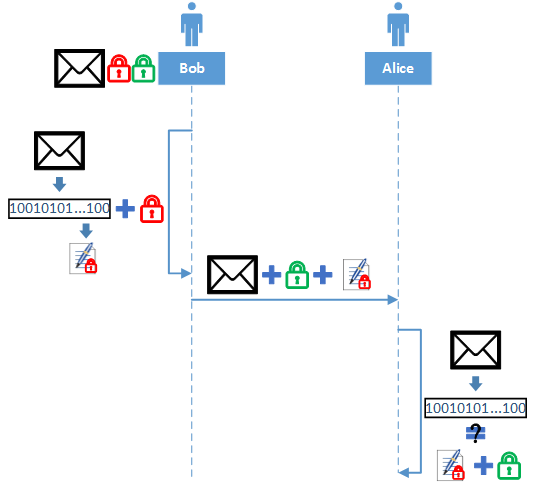
\includegraphics[width=0.7\textwidth]{img/signature.png}
	\caption{Échange d'un message signé}
	\label{signature}
\end{figure}

%%%%%%%%%%%%%%%%%%%%%%%%%%%%%%%%%%%%%%%%%%%%%%%%%%%%%%%%%%%%%%%%%%%%%%%%%%%

\subsubsection{Le certificat}

Un certificat est composé de :
\begin{itemize}
	\item une clé publique, et éventuellement la clé privée associée ;
	\item des informations sur le propriétaire ;
	\item une signature.
\end{itemize}

Les certificats sont signés par une autorité de certification, aussi appelé CA pour Certificat Autority, qui permet de garantir l'authenticité des certificats.
Seule l'autorité de certification racine est auto-signée.

%%%%%%%%%%%%%%%%%%%%%%%%%%%%%%%%%%%%%%%%%%%%%%%%%%%%%%%%%%%%%%%%%%%%%%%%%%%

\subsubsection{La PKI}

Une \textit{infrastructure à clés publiques}, aussi appelé par son terme anglais \textit{public key infrastructure}, permet la gestion de grandes quantités de certificats ou clés publiques.
Elle fournie des services de création, de publication et de révocation de certificats.
Cette infrastructure est principalement dans les systèmes informatiques utilisant de nombreux certificats.

%%%%%%%%%%%%%%%%%%%%%%%%%%%%%%%%%%%%%%%%%%%%%%%%%%%%%%%%%%%%%%%%%%%%%%%%%%%
%%%%%%%%%%%%%%%%%%%%%%%%%%%%%%%%%%%%%%%%%%%%%%%%%%%%%%%%%%%%%%%%%%%%%%%%%%%
%%%%%%%%%%%%%%%%%%%%%%%%%%%%%%%%%%%%%%%%%%%%%%%%%%%%%%%%%%%%%%%%%%%%%%%%%%%

\subsection{EJBCA}

%%%%%%%%%%%%%%%%%%%%%%%%%%%%%%%%%%%%%%%%%%%%%%%%%%%%%%%%%%%%%%%%%%%%%%%%%%%

\subsubsection{Utilisation dans Sides}

En production, le projet Sides utilise de nombreux certificats pour sécuriser les données.
Pour cela une PKI est utilisée permettant la gestion des nombreux certificats.

Lorsque l'on souhaite tester l'application avant la mise en production, il est nécessaire de pouvoir produire des certificats.
La mise en place d'une PKI peut s'avérer fastidieuse à intégrer et paramétrer pour fournir les mêmes services que la PKI de production.

Pour cela une PKI a été déployée sur les serveurs de tests, fournissant ainsi les fonctionnalités minimales utiles, notamment la production de certificats.
La PKI open-source EJBCA est utilisée par l'équipe Sides et le client pour gérer des certificats de test.

%%%%%%%%%%%%%%%%%%%%%%%%%%%%%%%%%%%%%%%%%%%%%%%%%%%%%%%%%%%%%%%%%%%%%%%%%%%

\subsubsection{Documentation}

Mon second objectif dans l'équipe Sides a été de rédiger une documentation de production de certificats en utilisant EJBCA.
Ces certificats doivent respecter les spécifications d'ICAO\footnote{ICAO - Site web : \url{http://www.icao.int}}, International Civil Aviation Organization, qui définissent les procédures et conseils destinés aux états et fournisseurs de solutions de PKI.

La documentation sera utilisée par le client pour produire ses certificats de tests.
Elle devait donc être la plus précise possible, détaillant toutes les étapes de la création, en spécifiant chacun des paramètres et options.
\\

Un profil définie les paramètres que les certificats, qui l'implémentent, devront définir.
J'ai tout d'abord créé deux profils qui seront utilisés pour le CSCA et le DS.

Le \textit{CSCA}, pour Country Signing Certificate Autority, est le certificat de plus haut niveau, utilisé par le le pays.
Il s'agit plus du plus critique car de lui dépend tous les autres certificats utilisés.
Dans certains pays, celui-ci est stocké dans un ordinateur portable situé dans un coffre fort, qui est ouvert en cas de besoin notamment lors du renouvellement des certificats.

Le \textit{DS}, pour Document Signer, est utilisé pour signer les documents sécurisés.
Il est situé au second niveau dans la hiérarchie des certificats, et est signé par le certificat racine CSCA.

Des certificats, composés d'une clé publique et une clé privée, peuvent ensuite être créés.
Ils peuvent être téléchargés sous le format PKCS\#12 qui est un fichier à l'extension ".p12".
L'utilisateur peut ensuite l'utiliser ou l'installer sur son environnement.

La figure \ref{hierarchie_CSCA_DS} représente la hiérarchie des différents certificats utilisés.
\begin{figure}[!h]
	\center
	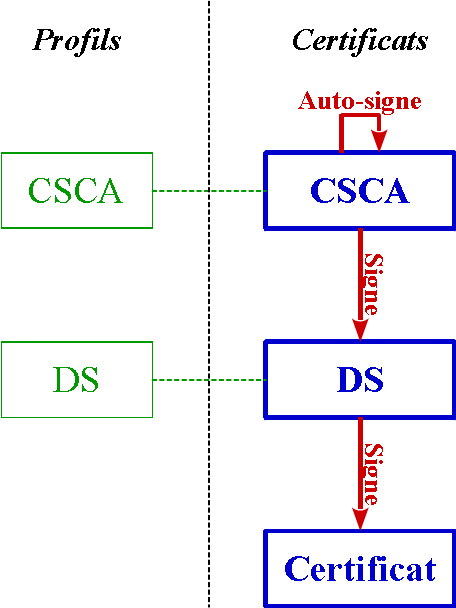
\includegraphics[width=0.5\textwidth]{img/hierarchie_CSCA_DS.png}
	\caption{Hiérarchie des certificats}
	\label{hierarchie_CSCA_DS}
\end{figure}

%%%%%%%%%%%%%%%%%%%%%%%%%%%%%%%%%%%%%%%%%%%%%%%%%%%%%%%%%%%%%%%%%%%%%%%%%%%
%%%%%%%%%%%%%%%%%%%%%%%%%%%%%%%%%%%%%%%%%%%%%%%%%%%%%%%%%%%%%%%%%%%%%%%%%%%
%%%%%%%%%%%%%%%%%%%%%%%%%%%%%%%%%%%%%%%%%%%%%%%%%%%%%%%%%%%%%%%%%%%%%%%%%%%

\subsection{Le SOD}

Le \textit{SOD}, Document Security Object, est la signature d'un document.
Cette signature est générée en utilisant la clé privée d'un certificat de type DS, présenté dans la section précédente.

Dans ce cadre j'ai travaillé sur le SOD des cartes à puce, plus particulièrement sur la création de la signature.
Ces cartes à puces contiennent :
\begin{enumerate}
	\item des données, disposées dans seize groupes (DG, pour Data Group), contenant les informations comme l'identité et la photo d'une personne ;
	\item la signature des données appelée SOD, créée à partir des différents DG et d'un certificat.
\end{enumerate}

Le SOD permet de vérifier que les données de la carte à puce n'ont pas été modifiées ou altérées.
Le processus de vérification est similaire à la vérification de la signature d'un message présenté dans la section \ref{La signature} :
\begin{itemize}
	\item On déchiffre le SOD avec la clé publique du DS ;
	\item On hache les données contenues dans les DGs ;
	\item Si les deux valeurs sont égales alors les données sont correctes.
\end{itemize}

%%%%%%%%%%%%%%%%%%%%%%%%%%%%%%%%%%%%%%%%%%%%%%%%%%%%%%%%%%%%%%%%%%%%%%%%%%%

\subsubsection{Documentation de fonctionnement}
\label{Documentation de fonctionnement}

Dans ce contexte, j'ai rédigé une documentation permettant d'expliquer comment créer la signature à partie des différents groupes de données (DG).
La création utilise une application web qui prend en paramètre les valeurs hexadécimales des groupes de données.
La signature est ensuite retournée sous la forme d'un fichier binaire.
Le figure \ref{processus_SOD} schématise le processus de création de la signature SOD.
\begin{figure}[!h]
	\center
	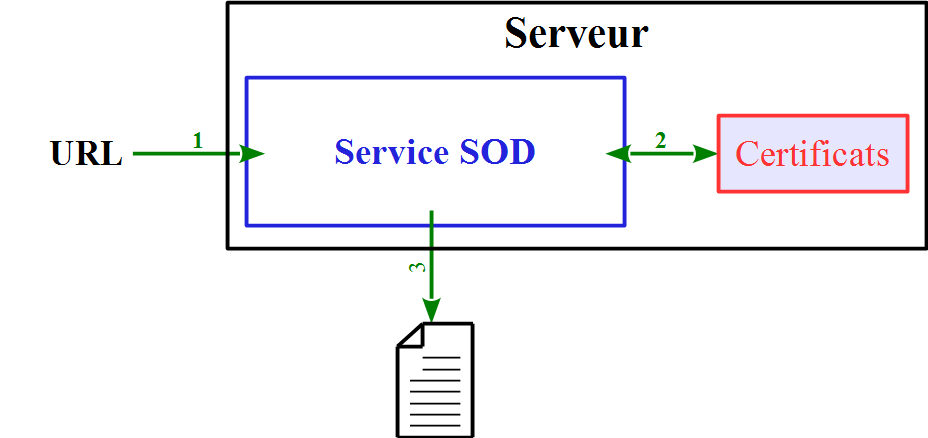
\includegraphics[width=0.8\textwidth]{img/processus_SOD.png}
	\caption{Processus de création du SOD}
	\label{processus_SOD}
\end{figure}

Une page HTML, dont une capture d'écran est présente sur la figure \ref{saisie_DGs}, permet de faciliter la saisie manuelle des données et l'appel au service en proposant respectivement des zones de saisie et un bouton de soumission.
La fenêtre de téléchargement s'affiche ensuite pour proposer d'ouvrir ou de sauvegarder le fichier constituant la signature.
\begin{figure}[!h]
	\center
	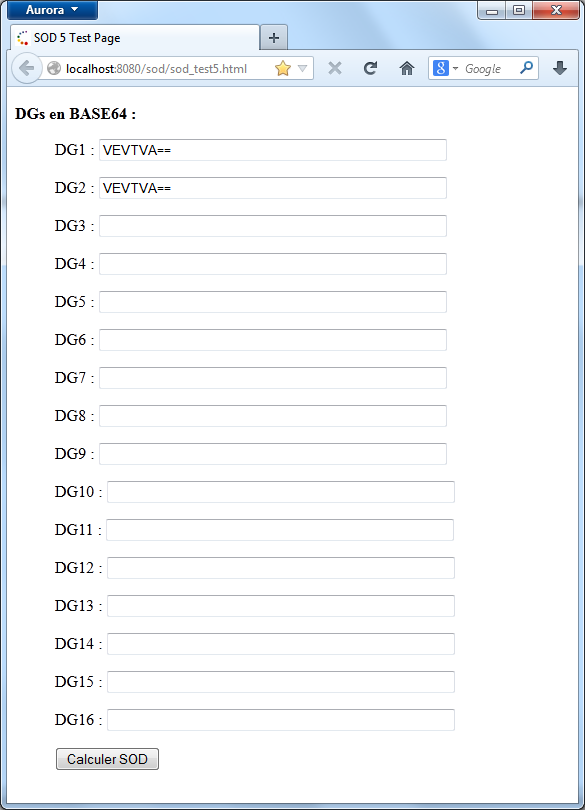
\includegraphics[width=0.6\textwidth]{img/saisie_DGs.png}
	\caption{Page HTML de saisie des groupes de données}
	\label{saisie_DGs}
\end{figure}

Il est aussi possible d'appeler le service de manière automatique depuis un programme.
Pour expliquer cela j'ai développé un exemple de script Python permettant de générer une signature.
\begin{lstlisting}[language = sh]
import urllib

# parameters
params = urllib.urlencode({"dataGroup1": "02468ACE",
                           "dataGroup2": "13579BDF"})

# invoke with POST parameters
dataPOST = urllib.urlopen("http://localhost:8080/sod", params)

# saving SOD
fileSOD = open("D:\\Desktop\\sod.out", 'w')
fileSOD.write(dataPOST.read())
fileSOD.close()

dataPOST.close()
\end{lstlisting}

%%%%%%%%%%%%%%%%%%%%%%%%%%%%%%%%%%%%%%%%%%%%%%%%%%%%%%%%%%%%%%%%%%%%%%%%%%%

\subsubsection{Application de test}

L'application web de création de signature est développée en JEE (Java Enterprise Edition).
Une \textit{servlet} est une classe java appelée lors d'une requête HTTP et permet de générer dynamiquement des données (généralement des pages HTML).
Le projet web fournie plusieurs servlets permettant d'utiliser plusieurs méthodes de signature, comme la connexion à un HSM (Hardware Security Module) ou l'utilisation de certificat PKCS\#12 décrit précédemment.

Dans l'objectif de fournir au client une application permettant de tester la création de signature SOD à partir d'un certificat PKCS\#12, j'ai modifié le projet web initial pour ne garder que la fonctionnalité correspondante.
L'épuration du code source et la correction de certains bugs ont permis de produire une solution fonctionnelle qui fourni les services de signature de données décrites dans la partie \ref{Documentation de fonctionnement}.